\section{Git 核心命令场景全解}
\textbf{核心摘要:}  
分类解析 Git 工作流各阶段关键命令,覆盖仓库管理、版本控制、分支操作与团队协作场景。

\subsection{仓库与初始化}
\begin{center}
\begin{tabular}{llp{8cm}}
    \toprule
    \textbf{命令} & \textbf{场景} & \textbf{说明} \\
    \midrule
    \texttt{git init} & 新建项目 & 初始化本地仓库(创建 \texttt{.git} 目录) \\
    \texttt{git clone <url>} & 获取远程项目 & 克隆远程仓库到本地(含完整历史) \\
    \texttt{git remote add <名> <url>} & 关联远程仓库 & 添加远程别名(通常命名为 \texttt{origin}) \\
    \texttt{git config --global user.*} & 全局设置 & 配置用户名/邮箱(首次使用必需) \\
    \bottomrule
\end{tabular}
\end{center}

\subsection{日常开发流程}
\begin{center}
\begin{tabular}{llp{8cm}}
    \toprule
    \textbf{命令} & \textbf{场景} & \textbf{说明} \\
    \midrule
    \texttt{git status} & 查看工作状态 & 显示暂存/未跟踪文件(每日高频使用) \\
    \texttt{git add <文件>} & 准备提交 & 添加文件到暂存区(\texttt{git add .} 添加所有) \\
    \texttt{git commit -m "说明"} & 创建版本 & 提交暂存区内容到本地仓库(原子化修改) \\
    \texttt{git diff} & 代码审查 & 查看未暂存的修改内容(避免错误提交) \\
    \texttt{git restore <文件>} & 撤销修改 & 丢弃工作区未暂存的更改(危险操作前备份) \\
    \bottomrule
\end{tabular}
\end{center}

\subsection{分支管理策略}
\begin{center}
\begin{tabular}{llp{8cm}}
    \toprule
    \textbf{命令} & \textbf{场景} & \textbf{说明} \\
    \midrule
    \texttt{git branch <名>} & 功能开发 & 创建新分支(隔离开发环境) \\
    \texttt{git checkout <分支>} & 切换上下文  & 切换分支(\texttt{git checkout -b} 创建并切换) \\
    \texttt{git merge <分支>} & 集成功能 & 合并指定分支到当前分支(产生合并提交) \\
    \texttt{git rebase <分支>} & 整理历史 & 变基分支(线性提交历史,需谨慎使用) \\
    \texttt{git branch -d <分支>} & 清理环境 & 删除已合并分支(保持仓库整洁) \\
    \bottomrule
\end{tabular}
\end{center}

\subsection{远程协作}
\begin{center}
\begin{tabular}{llp{8cm}}
    \toprule
    \textbf{命令} & \textbf{场景} & \textbf{说明} \\
    \midrule
    \texttt{git fetch} & 安全更新 & 获取远程变更(不自动合并) \\
    \texttt{git pull} & 快速同步 & 拉取远程变更并合并(\texttt{= fetch + merge}) \\
    \texttt{git push} & 发布代码 & 推送本地提交到远程(首次需 \texttt{-u} 关联) \\
    \texttt{git push -f} & 紧急修复 & 强制覆盖远程(仅限私有分支,团队慎用) \\
    \texttt{git remote -v} & 诊断问题 & 查看远程仓库配置(排查推送失败) \\
    \bottomrule
\end{tabular}
\end{center}

\subsection{历史与版本}
\begin{center}
\begin{tabular}{llp{8cm}}
    \toprule
    \textbf{命令} & \textbf{场景} & \textbf{说明} \\
    \midrule
    \texttt{git log} & 审计追踪 & 查看提交历史(\texttt{--oneline} 简洁模式) \\
    \texttt{git blame <文件>} & 追溯责任 & 显示文件每行最后修改者 \\
    \texttt{git tag v1.0} & 版本发布 & 创建版本标签(标记重要里程碑) \\
    \texttt{git checkout <哈希>} & 问题排查 & 切换到历史版本(临时回退测试) \\
    \texttt{git bisect} & 定位缺陷 & 二分法查找引入 Bug 的提交 \\
    \bottomrule
\end{tabular}
\end{center}

\subsection{撤销与修复}
\begin{center}
\begin{tabular}{llp{8cm}}
    \toprule
    \textbf{命令} & \textbf{场景} & \textbf{说明} \\
    \midrule
    \texttt{git reset <模式>} & 撤销提交 & \begin{tabular}[t]{@{}l@{}} \texttt{--soft}:保留修改 \\ \texttt{--hard}:彻底删除 \end{tabular}
 \\
    \texttt{git commit --amend} & 快速修正 & 修改最近提交(未推送时使用) \\
    \texttt{git revert <提交>} & 安全回退 & 创建新提交撤销指定修改(已推送时使用) \\
    \texttt{git stash} & 暂存变更 & 临时保存工作区(切换分支前必备) \\
    \texttt{git reflog} & 灾难恢复 & 查看所有操作记录(找回误删分支/提交) \\
    \bottomrule
\end{tabular}
\end{center}

\subsection{配置与优化}
\begin{center}
\begin{tabular}{llp{8cm}}
    \toprule
    \textbf{命令} & \textbf{场景} & \textbf{说明} \\
    \midrule
    \texttt{git config alias.*} & 提升效率 & 创建命令别名(如 \texttt{co = checkout}) \\
    \texttt{git ignore} & 规范管理 & 生成 \texttt{.gitignore} 模板(排除临时文件) \\
    \texttt{git gc} & 仓库维护 & 清理优化仓库(减少磁盘占用) \\
    \texttt{git worktree} & 并行开发 & 多工作目录操作(同时开发多个分支) \\
    \texttt{git submodule} & 依赖管理 & 嵌套其他仓库(第三方库集成) \\
    \bottomrule
\end{tabular}
\end{center}

\subsection{命令使用频率统计}
\begin{center}
\begin{tikzpicture}
\begin{axis}[
    ybar,
    xlabel={命令类别},
    ylabel={使用频率},
    symbolic x coords={日常开发,分支管理,远程协作,历史查看},
    xtick=data,
    nodes near coords,
    bar width=15pt
]
\addplot coordinates {
    (日常开发,85) 
    (分支管理,70)
    (远程协作,65)
    (历史查看,40)
};
\end{axis}
\end{tikzpicture}
\end{center}

\textbf{黄金法则:}
\begin{itemize}[leftmargin=*, nosep]
    \item 提交前必查 \texttt{git status} 和 \texttt{git diff}
    \item 推送前执行 \texttt{git pull} 避免冲突
    \item 修改已推送历史用 \texttt{git revert} 替代 \texttt{reset}
    \item 功能开发必建新分支
\end{itemize}


\section{本地仓库与远程仓库核心区别解析}
\textbf{核心摘要:}  
本地仓库存储于开发者机器实现离线操作,远程仓库部署于服务器支持团队协作,两者通过同步机制保持版本统一。

\subsection{基础特性对比}
\begin{center}
\begin{tabular}{lcc}
    \toprule
    \textbf{特性} & \textbf{本地仓库} & \textbf{远程仓库} \\
    \midrule
    物理位置 & 开发者计算机 & 云服务器(GitHub/GitLab等) \\
    存储内容 & 完整项目历史 + 工作目录 & 仅版本库(无工作目录) \\
    访问方式 & 本地文件系统 & HTTPS/SSH网络协议 \\
    核心文件 & \texttt{.git}目录 + 项目文件 & 仅\texttt{.git}数据包 \\
    创建方式 & \texttt{git init} 或 \texttt{git clone} & Web平台创建 + \texttt{git push} \\
    \bottomrule
\end{tabular}
\end{center}

\subsection{功能定位差异}
\begin{itemize}[leftmargin=*, nosep]
    \item \textbf{本地仓库核心功能}
    \begin{itemize}
        \item 版本控制:\texttt{commit}/\texttt{branch}/\texttt{tag}操作
        \item 开发环境:实时编辑文件
        \item 离线工作:无网络时继续开发
        \item 实验场:安全执行危险操作
    \end{itemize}
    
    \item \textbf{远程仓库核心功能}
    
\begin{itemize}
        \item 中央存储:团队代码统一管理
        \item 协作枢纽:Pull Request/Code Review
        \item 持续集成:触发CI/CD流水线
        \item 灾备中心:防止本地数据丢失
    \end{itemize}
\end{itemize}

\subsection{操作机制对比}
\begin{center}
\begin{tabular}{lll}
    \toprule
    \textbf{操作类型} & \textbf{本地仓库命令} & \textbf{远程仓库交互} \\
    \midrule
    提交更新 & \texttt{git commit} & 无直接操作 \\
    创建分支 & \texttt{git branch} & 推送后自动同步 \\
    查看历史 & \texttt{git log} & Web界面查看 \\
    代码合并 & \texttt{git merge} & Pull Request流程 \\
    版本恢复 & \texttt{git reset} & 强制推送覆盖 \\
    \bottomrule
\end{tabular}
\end{center}

\subsection{同步机制详解}
\begin{enumerate}[leftmargin=*, nosep]
    \item \textbf{数据流向}
    \begin{itemize}[leftmargin=*, nosep]
        \item 推送(Push):\texttt{git push} → 本地 → 远程
        \item 拉取(Pull):\texttt{git pull} ← 远程 ← 本地
    \end{itemize}
    
    \item \textbf{同步频率}
    
\begin{itemize}[leftmargin=*, nosep]
        \item 本地:即时生效(提交即存版本)
        \item 远程:需显式推送(未推送内容他人不可见)
    \end{itemize}
    
    \item \textbf{冲突解决}
    
\begin{itemize}[leftmargin=*, nosep]
        \item 本地冲突:直接编辑文件解决
        \item 远程冲突:拉取后本地解决再推送
    \end{itemize}
\end{enumerate}

\subsection{存储结构差异}
\begin{center}
\begin{tikzpicture}
\node[draw, rounded corners, fill=blue!10, minimum width=3cm] (local) at (0,0) {
    \begin{tabular}{c}
        \textbf{本地仓库} \\
        \hline
        \texttt{/project/} \\
        ├── \textcolor{red}{工作目录} \\
        │   ├── src/ \\
        │   └── docs/ \\
        └── \texttt{.git/} \\
    \end{tabular}
};

\node[draw, rounded corners, fill=green!10, minimum width=3cm] (remote) at (5,0) {
    
\begin{tabular}{c}
        \textbf{远程仓库} \\
        \hline
        \texttt{repo.git/} \\
        ├── objects/ \\
        ├── refs/ \\
        ├── HEAD \\
        └── config \\
    \end{tabular}
};

\draw[->, thick] (local.east) -- node[above] {\texttt{git push}} (remote.west);
\draw[->, thick] (remote.west) -- node[below] {\texttt{git fetch}} (local.east);
\end{tikzpicture}
\end{center}

\subsection{最佳实践指南}
\begin{itemize}[leftmargin=*, nosep]
    \item \textbf{本地操作原则}
    \begin{itemize}[leftmargin=*, nosep]
        \item 功能开发在特性分支完成
        \item 每日工作结束前推送
        \item 敏感信息不进本地历史
    \end{itemize}
    
    \item \textbf{远程管理规范}
    
\begin{itemize}[leftmargin=*, nosep]
        \item \texttt{main}分支保护机制
        \item 强制Code Review流程
        \item 定期仓库镜像备份
    \end{itemize}
    
    \item \textbf{同步策略}
    
\begin{itemize}[leftmargin=*, nosep]
        \item 推送前先拉取(\texttt{git pull --rebase})
        \item 避免强制推送(\texttt{git push -f})
        \item 使用钩子自动化测试
    \end{itemize}
\end{itemize}

\subsection{典型应用场景}
\begin{center}
\begin{tabular}{lp{6cm}p{6cm}}
    \toprule
    \textbf{场景} & \textbf{本地仓库操作} & \textbf{远程仓库操作} \\
    \midrule
    新功能开发 & \texttt{git checkout -b feat/new} & 创建PR合并到\texttt{main} \\
    紧急修复 & \texttt{git commit --amend} & 创建hotfix分支 \\
    代码审查 & \texttt{git diff HEAD\~{}3} & 在PR页面评论 \\
    版本发布 & \texttt{git tag v1.0} & 生成Release包 \\
    \bottomrule
\end{tabular}
\end{center}

\section{Git Status 命令详解}
\textbf{一句话总结:}  
Git Status 用于实时展示工作目录与暂存区的状态变化,是版本控制中监测代码变更的核心诊断工具。

\subsection{核心功能与应用场景}
\begin{enumerate}[leftmargin=*, nosep]
    \item \textbf{状态诊断}  \\
    显示三类关键文件状态:
    \begin{itemize}[leftmargin=*, nosep]
        \item \textcolor{red}{已修改未暂存}:工作区改动但未执行 \texttt{git add}
        \item \textcolor{green}{已暂存待提交}:已 \texttt{add} 但未 \texttt{commit}
        \item \textcolor{gray}{未跟踪文件}:新创建未纳入版本控制
    \end{itemize}
    \textbf{使用场景}:开发中随时确认代码变更范围,避免提交遗漏
    
    \item \textbf{分支状态监控}  \\
    显示当前分支与远程分支的同步状态:
    
\begin{itemize}[leftmargin=*, nosep]
        \item 本地领先/落后远程提交数
        \item 当前分支关联的远程分支名
        \item 冲突预警(合并/变基后)
    \end{itemize}
    \textbf{使用场景}:推送前检查分支状态,避免推送冲突
    
    \item \textbf{操作指引}  \\
    根据当前状态输出下一步建议命令:
    
\begin{itemize}[leftmargin=*, nosep]
        \item 未暂存文件 → 提示 \texttt{git add <file>} 或 \texttt{git restore <file>}
        \item 无远程分支 → 提示 \texttt{git push -u origin <branch>}
        \item 冲突状态 → 提示解决冲突方法
    \end{itemize}
    \textbf{使用场景}:指导Git新手正确执行后续操作
\end{enumerate}

\subsection{实战应用示例}
\begin{enumerate}[leftmargin=*, nosep]
    \item \textbf{提交前检查} \\
    修改文件后执行:
    \begin{verbatim}
$ git status
位于分支 main
尚未暂存以备提交的变更:
  (使用 "git add <文件>..." 更新要提交的内容)
  (使用 "git restore <文件>..." 丢弃工作区的改动)
        修改:     index.html

未跟踪的文件:
  (使用 "git add <文件>..." 以包含要提交的内容)
        logo.png
    \end{verbatim}
    \textbf{操作决策}:需执行 \texttt{git add index.html logo.png}
    
    \item \textbf{分支同步确认} \\
    协作开发时执行:
    
\begin{verbatim}
$ git status
位于分支 feature/login
您的分支落后 'origin/feature/login' 共 2 个提交
  (使用 "git pull" 更新您的本地分支)
    \end{verbatim}
    \textbf{操作决策}:立即执行 \texttt{git pull} 避免冲突
    
    \item \textbf{冲突预警} \\
    合并分支后出现冲突:
    
\begin{verbatim}
$ git status
您有尚未合并的路径
  (解决冲突并运行 "git commit")
未合并的路径:
  (使用 "git add <文件>..." 标记解决方案)
        双方修改:   styles.css
    \end{verbatim}
    \textbf{操作决策}:手动解决 \texttt{styles.css} 冲突后标记为已解决
\end{enumerate}

\subsection{高级使用技巧}
\begin{center}
\begin{tabular}{ll}
    \toprule
    \textbf{参数} & \textbf{效果} \\
    \midrule
    \texttt{-s} & 精简模式输出(状态缩写) \\
    \texttt{--ignored} & 显示被忽略的文件 \\
    \texttt{-b} & 显示分支及跟踪信息 \\
    \texttt{--show-stash} & 显示暂存区内容 \\
    \bottomrule
\end{tabular}
\end{center}

\textbf{精简模式示例}:
\begin{verbatim}
$ git status -s
 M README.md      # 已修改未暂存
A  index.js       # 新添加已暂存
?? config.yaml    # 未跟踪文件
UU styles.css     # 冲突文件
\end{verbatim}

\subsection{最佳实践}
\begin{itemize}[leftmargin=*, nosep]
    \item \textbf{高频检查}:关键操作(提交/合并/推送)前必执行
    \item \textbf{组合使用}:配合 \texttt{git diff} 查看变更细节
    \item \textbf{自动化集成}:CI/CD 流水线中作为预检查步骤
    \item \textbf{团队规范}:代码评审前要求提供 \texttt{git status} 输出
\end{itemize}



\section{.git 目录结构与文件功能详解}
\textbf{一句话总结:}  
`.git` 目录是 Git 仓库的核心,存储版本控制的所有元数据(如提交历史、分支引用、对象数据库等),以下是对 `ls -al` 输出的详细解析。


\subsection{一、目录概览}
\begin{verbatim}
total 56# 目录总大小(单位:块)
drwxr-xr-x@ 14 player_he staff 448 8 26 20:06 .# 当前目录(.git)
drwx------@ 24 player_he staff 768 8 26 20:07 ..# 父目录(仓库根目录)
\end{verbatim}

\begin{itemize}[leftmargin=*, nosep]
    \item \textbf{权限说明}:\texttt{drwxr-xr-x@} 表示目录(\texttt{d}),所有者(\texttt{player\_he})有读/写/执行权限(\texttt{rwx}),组用户(\texttt{staff})和其他用户有读/执行权限(\texttt{r-x});\texttt{@} 表示文件带有 macOS 扩展属性(如 Finder 标签)。
    \item \textbf{时间说明}:\texttt{.git} 目录最后修改时间为 8月26日20:06,父目录为 20:07,说明近期有 Git 操作(如提交、推送)。
\end{itemize}


\subsection{二、核心文件解析}
\subsubsection{1. 提交相关文件}
\begin{verbatim}
-rw-r--r--@ 1 player_he staff 400 8 26 20:06 COMMIT_EDITMSG# 最近提交的消息缓存
\end{verbatim}

\begin{itemize}[leftmargin=*, nosep]
    \item \textbf{功能}:保存最近一次 \texttt{git commit} 时输入的提交信息(若使用编辑器编写)。
    \item \textbf{特点}:提交完成后不会自动删除,可用于恢复误删的提交消息。
\end{itemize}

\subsubsection{2. 仓库配置文件}
\begin{verbatim}
-rw-r--r-- 1 player_he staff 186 8 26 18:43 config# 仓库本地配置
\end{verbatim}

\begin{itemize}[leftmargin=*, nosep]
    \item \textbf{功能}:存储仓库-specific 的配置(如用户信息、远程仓库地址、分支关联等)。
    \item \textbf{示例内容}:
    \begin{verbatim}
[remote "origin"]
url = https://github.com/your-name/repo.git
fetch = +refs/heads/*:refs/remotes/origin/*
[branch "main"]
remote = origin
merge = refs/heads/main
    \end{verbatim}
    \item \textbf{修改时间}:8月26日18:43,说明近期修改过仓库配置(如添加远程仓库)。
\end{itemize}

\subsubsection{3. 仓库描述文件}
\begin{verbatim}
-rw-r--r--@ 1 player_he staff 73 8 26 11:20 description# 仓库描述
\end{verbatim}

\begin{itemize}[leftmargin=*, nosep]
    \item \textbf{功能}:存储仓库的 human-readable 描述(如“我的项目”),主要用于 GitWeb 或 GitHub 等平台显示。
    \item \textbf{特点}:默认内容为 `Unnamed repository; edit this file 'description' to name the repository.`,可手动修改。
\end{itemize}

\subsubsection{4. 远程同步记录}
\begin{verbatim}
-rw-r--r--@ 1 player_he staff 102 8 26 11:39 FETCH_HEAD# 最近 fetch 操作的结果
\end{verbatim}

\begin{itemize}[leftmargin=*, nosep]
    \item \textbf{功能}:记录最近一次 \texttt{git fetch} 从远程仓库获取的分支头提交(如 \texttt{origin/main} 的最新哈希)。
    \item \textbf{示例内容}:
    \begin{verbatim}
8a3f5e9... refs/heads/main from origin
    \end{verbatim}
\end{itemize}

\subsubsection{5. 当前分支引用}
\begin{verbatim}
-rw-r--r--@ 1 player_he staff 21 8 26 12:06 HEAD# 当前分支指针
\end{verbatim}

\begin{itemize}[leftmargin=*, nosep]
    \item \textbf{功能}:指向当前所在的分支(或提交),是 Git 工作流程的核心指针。
    \item \textbf{示例内容}:
    \begin{verbatim}
ref: refs/heads/main# 表示当前在 main 分支
    \end{verbatim}
    \item \textbf{修改时间}:8月26日12:06,说明近期切换过分支(如 \texttt{git checkout main})。
\end{itemize}

\subsubsection{6. 暂存区(Index)文件}
\begin{verbatim}
-rw-r--r--@ 1 player_he staff 1892 8 26 20:06 index# 暂存区数据库
\end{verbatim}

\begin{itemize}[leftmargin=*, nosep]
    \item \textbf{功能}:记录当前要提交的文件快照(即“暂存区”状态),包含文件名、权限、哈希值等信息。
    \item \textbf{作用}:\texttt{git add} 命令将文件添加到此处,\texttt{git commit} 命令将此处的内容提交到对象数据库。
    \item \textbf{大小说明}:1892字节,说明暂存区中有多个文件等待提交。
\end{itemize}

\subsubsection{7. 分支/标签引用目录}
\begin{verbatim}
drwxr-xr-x@ 5 player_he staff 160 8 26 11:39 refs# 引用存储目录
\end{verbatim}

\begin{itemize}[leftmargin=*, nosep]
    \item \textbf{子目录}:
    \begin{itemize}[leftmargin=*, nosep]
        \item \texttt{refs/heads/}:存储本地分支的指针(如 \texttt{main}、\texttt{feature/login});
        \item \texttt{refs/tags/}:存储标签的指针(如 \texttt{v1.0});
        \item \texttt{refs/remotes/}:存储远程分支的指针(如 \texttt{origin/main})。
    \end{itemize}
    \item \textbf{功能}:通过文本文件记录分支/标签的最新提交哈希(如 \texttt{refs/heads/main} 内容为 \texttt{8a3f5e9...})。
\end{itemize}


\subsection{三、核心文件夹解析}
\subsubsection{1. 对象数据库(Objects)}
\begin{verbatim}
drwxr-xr-x@ 75 player_he staff 2400 8 26 20:06 objects# 对象存储目录
\end{verbatim}

\begin{itemize}[leftmargin=*, nosep]
    \item \textbf{功能}:存储 Git 所有版本的数据(**对象数据库**),包含四类对象:
    \begin{itemize}[leftmargin=*, nosep]
        \item \textbf{Blob}:文件内容(如 \texttt{index.html} 的内容);
        \item \textbf{Tree}:目录结构(如 \texttt{src/} 目录下的文件列表);
        \item \textbf{Commit}:提交记录(如作者、时间、父提交、树对象哈希);
        \item \textbf{Tag}:标签对象(如 \texttt{v1.0} 的描述)。
    \end{itemize}
    \item \textbf{结构}:采用哈希前缀目录(如 \texttt{8a/3f5e9...})存储,提高检索效率。
    \item \textbf{大小说明}:2400字节,75个项目,说明仓库有较多版本数据(如多次提交)。
\end{itemize}

\subsubsection{2. 钩子脚本(Hooks)}
\begin{verbatim}
drwxr-xr-x@ 16 player_he staff 512 8 26 13:46 hooks# 钩子脚本目录
\end{verbatim}

\begin{itemize}[leftmargin=*, nosep]
    \item \textbf{功能}:存储 Git 事件触发的脚本(如 \texttt{pre-commit}、\texttt{post-push}),用于自动化流程(如代码检查、测试)。
    \item \textbf{默认脚本}:包含 \texttt{pre-commit.sample}、\texttt{post-commit.sample} 等示例脚本,需移除 \texttt{.sample} 后缀才会生效。
    \item \textbf{修改时间}:8月26日13:46,说明近期可能添加或修改过钩子脚本。
\end{itemize}

\subsubsection{3. 日志目录(Logs)}
\begin{verbatim}
drwxr-xr-x@ 4 player_he staff 128 8 26 11:31 logs# 操作日志目录
\end{verbatim}

\begin{itemize}[leftmargin=*, nosep]
    \item \textbf{功能}:存储分支/远程分支的操作日志(如 \texttt{git commit}、\texttt{git merge} 的历史)。
    \item \textbf{子文件}:\texttt{logs/refs/heads/main} 记录 \texttt{main} 分支的所有提交历史;\texttt{logs/refs/remotes/origin/main} 记录远程 \texttt{origin/main} 分支的同步历史。
    \item \textbf{作用}:用于恢复误删的分支(如 \texttt{git reflog} 命令读取此处的日志)。
\end{itemize}

\subsubsection{4. 信息目录(Info)}
\begin{verbatim}
drwxr-xr-x@ 3 player_he staff 96 8 26 11:20 info# 额外信息目录
\end{verbatim}

\begin{itemize}[leftmargin=*, nosep]
    \item \textbf{子文件}:\texttt{info/exclude},用于记录不希望 Git 跟踪的文件(类似 \texttt{.gitignore},但不会提交到仓库)。
    \item \textbf{用途}:存储本地临时文件(如 \texttt{*.log}、\texttt{tmp/})的忽略规则。
\end{itemize}


\subsection{四、关键文件总结}
\begin{center}
\begin{tabular}{@{}lll@{}}
\toprule
文件/目录       & 核心功能                              & 关联命令                \\
\midrule
\texttt{config} & 仓库配置                              & \texttt{git config}     \\
\texttt{HEAD}   & 当前分支指针                          & \texttt{git checkout}   \\
\texttt{index}  & 暂存区                                & \texttt{git add}、\texttt{git commit} \\
\texttt{objects} & 对象数据库(所有版本数据)            & \texttt{git commit}、\texttt{git merge} \\
\texttt{refs}   & 分支/标签引用                          & \texttt{git branch}、\texttt{git tag} \\
\texttt{logs}   & 操作日志                              & \texttt{git reflog}     \\
\texttt{hooks}  & 自动化钩子脚本                        & \texttt{git commit}、\texttt{git push} \\
\bottomrule
\end{tabular}
\end{center}


\subsection{五、注意事项}
\begin{itemize}[leftmargin=*, nosep]
    \item \textbf{不要手动修改}:\texttt{.git} 目录中的文件(如 \texttt{objects}、\texttt{refs})由 Git 自动管理,手动修改可能导致仓库损坏。
    \item \textbf{备份重要文件}:\texttt{config}、\texttt{HEAD}、\texttt{refs} 等文件包含仓库的关键配置,建议定期备份。
    \item \textbf{理解权限}:\texttt{rw-r--r--} 表示所有者可读写,其他人只读,确保仓库安全(避免他人修改配置)。
\end{itemize}


通过以上解析,可清晰了解 \texttt{.git} 目录的结构与每个文件的功能,这是理解 Git 版本控制原理的关键。


\section{Git Add 命令详解}
\textbf{一句话总结:}  
`git add` 是 Git 工作流的核心命令,用于将工作目录的变更添加到暂存区(Staging Area),为提交做准备。

\subsection{核心功能解析}
\begin{itemize}[leftmargin=*, nosep]
    \item \textbf{暂存变更}:将文件修改/新增/删除操作记录到索引区
    \item \textbf{精确控制}:选择性添加特定文件或部分修改
    \item \textbf{版本快照}:创建待提交的精确文件状态
    \item \textbf{冲突管理}:标记冲突解决后的文件状态
\end{itemize}

\subsection{四大应用场景与示例}
\begin{enumerate}[leftmargin=*, nosep]
    \item \textbf{添加新文件} \\
    \texttt{\$ touch index.html} \quad \textcolor{gray}{// 创建新文件} \\
    \texttt{\$ git add index.html} \quad \textcolor{gray}{// 纳入版本控制}
    
    \item \textbf{暂存修改文件} \\
    \texttt{\$ echo "content" > README.md} \quad \textcolor{gray}{// 修改文件} \\
    \texttt{\$ git add README.md} \quad \textcolor{gray}{// 准备提交}
    
    \item \textbf{添加目录下所有变更} \\
    \texttt{\$ git add .} \quad \textcolor{gray}{// 添加当前目录所有变更} \\
    \texttt{\$ git add src/} \quad \textcolor{gray}{// 添加特定目录变更}
    
    \item \textbf{交互式暂存(精细控制)} \\
    \texttt{\$ git add -p} \\
    \textcolor{gray}{// 进入交互模式,逐块选择修改内容}
\end{enumerate}

\subsection{工作流位置图示}
\begin{center}
\begin{tikzpicture}[node distance=2cm]
\node (work) [draw, fill=blue!10] {工作目录};
\node (stage) [draw, fill=green!10, right of=work] {暂存区};
\node (repo) [draw, fill=red!10, right of=stage] {本地仓库};

\draw [->, thick] (work) -- node[above] {\texttt{git add}} (stage);
\draw [->, thick] (stage) -- node[above] {\texttt{git commit}} (repo);
\end{tikzpicture}
\end{center}

\subsection{高级使用技巧}
\begin{center}
\begin{tabular}{@{}ll@{}}
    \toprule
    \textbf{命令} & \textbf{功能} \\
    \midrule
    \texttt{git add -u} & 添加所有已跟踪文件的修改(不含新文件) \\
    \texttt{git add -A} & 添加所有变更(包括删除操作) \\
    \texttt{git add -i} & 进入交互式暂存菜单 \\
    \texttt{git add -p <file>} & 对特定文件进行块级选择 \\
    \texttt{git add -N <file>} & 预备添加(标记新文件但暂不包含内容) \\
    \bottomrule
\end{tabular}
\end{center}

\subsection{典型错误场景处理}
\begin{enumerate}[leftmargin=*, nosep]
    \item \textbf{误添加文件} \\
    \texttt{\$ git reset HEAD <file>} \quad \textcolor{gray}{// 从暂存区移除}
    
    \item \textbf{添加大文件} \\
    \texttt{\$ git reset HEAD bigfile.zip} \\
    \texttt{\$ echo "bigfile.zip" >> .gitignore} \quad \textcolor{gray}{// 避免再次添加}
    
    \item \textbf{部分文件不提交} \\
    \texttt{\$ git add -p} \quad \textcolor{gray}{// 交互模式选择需要片段}
\end{enumerate}

\subsection{最佳实践指南}
\begin{itemize}[leftmargin=*, nosep]
    \item \textbf{小步提交}:多次 \texttt{add} + 单次 \texttt{commit}(原子化修改)
    \item \textbf{审查变更}:\texttt{add} 前执行 \texttt{git diff} 确认修改
    {diff} 确认修改
    \item \textbf{忽略机制}:配置 \texttt{.gitignore} 避免添加临时文件
    \item \textbf{安全操作}:敏感数据误添加时立即 \texttt{git reset}
\end{itemize}

\subsection{工作流示例:功能开发}
\begin{verbatim}
# 1. 创建新功能分支
git checkout -b feature/login

# 2. 修改登录模块
vim login.js
vim login.css

# 3. 选择性暂存
git add login.js      # 先提交JS修改
git commit -m "实现登录验证逻辑"

# 4. 添加CSS修改
git add login.css
CSS修改
git add login.css
git commit -m "添加登录页样式"

# 5. 推送分支
git push origin feature/login
\end{verbatim}

\section{Git Commit 命令详解}
\textbf{一句话总结:}  
`git commit` 是 Git 版本控制的核心命令,用于将暂存区的变更永久保存到本地仓库,创建可追溯的代码历史记录。

\subsection{核心功能解析}
\begin{itemize}[leftmargin=*, nosep]
    \item \textbf{版本快照}:捕获暂存区的精确状态
    \item \textbf{历史记录}:生成带时间戳的提交记录
    \item \textbf{元数据存储}:记录作者、提交者、时间等信息
    \item \textbf{分支演进}:推进当前分支指针到新提交
\end{itemize}

\subsection{五大应用场景与示例}
\begin{enumerate}[leftmargin=*, nosep]
    \item \textbf{基础提交} \\ 
    \texttt{git add index.html} \quad \textcolor{gray}{// 暂存修改}  
    \texttt{\$ git commit -m "修复登录页面布局"} \\
    \textcolor{gray}{→ 创建包含指定消息的提交}
    
    \item \textbf{多文件原子提交} \\
    \texttt{\$ git add user-service.js user-model.js} \\
    \texttt{\$ git commit -m "实现用户注册功能"} \\
    \textcolor{gray}{→ 将相关修改作为整体提交}
    
    \item \textbf{紧急修复提交} \\
    \texttt{\$ git commit -am "热修复:解决空指针异常"} \\
    \textcolor{gray}{→ \texttt{-a} 参数自动暂存已跟踪文件的修改}
    
    \item \textbf{空提交(CI/CD触发)} \\
    \texttt{\$ git commit --allow-empty -m "触发部署流水线"} \\
    \textcolor{gray}{→ 创建无内容变更的提交}
    
    \item \textbf{提交关联问题追踪} \\
    \texttt{\$ git commit -m "优化数据库查询 \#JIRA-123"} \\
    \textcolor{gray}{→ 在消息中关联工单系统}
\end{enumerate}

% 修复后的工作流位置图示(匹配右侧效果)
\subsubsection{工作流位置图示}  % 标题级别:对应右侧0.6.3(subsubsection)
\begin{center}                 % 居中显示图示
  \begin{tikzpicture}[
    node distance=2.5cm,        % 节点间距
    every node/.style={draw, thick, minimum size=1.2cm}  % 节点默认样式(边框、厚度、最小尺寸)
  ]
    % 定义节点(从左到右排列)
    \node(work)[fill=blue!10]   {工作目录};                  % 工作目录:浅蓝色填充
    \node(stage)[fill=green!10, right of=work] {暂存区};    % 暂存区:绿色填充,在work右侧
    \node(repo)[fill=red!10, right of=stage]  {本地仓库};  % 本地仓库:红色填充,在stage右侧
    \node(remote)[fill=orange!10, right of=repo] {远程仓库};% 远程仓库:橙色填充,在repo右侧

    % 绘制箭头及命令(从左到右)
    \draw[->, thick] (work) -- node[above] {\texttt{git add}} (stage);    % 工作目录→暂存区:git add
    \draw[->, thick] (stage) -- node[above] {\texttt{git commit}} (repo); % 暂存区→本地仓库:git commit
    \draw[->, thick] (repo) -- node[above] {\texttt{git push}} (remote);  % 本地仓库→远程仓库:git push
  \end{tikzpicture}
\end{center}



\subsection{高级使用技巧}
\begin{center}
\begin{tabular}{@{}ll@{}}
    \toprule
    \textbf{命令} & \textbf{功能} \\
    \midrule
    \texttt{git commit --amend} & 修改最近提交(消息/内容) \\
    \texttt{git commit -v} & 提交时显示变更差异 \\
    \texttt{git commit --date="2023-01-01"} & 自定义提交时间 \\
    \texttt{git commit -S} & GPG签名提交 \\
    \texttt{git commit -C HEAD} & 重用上次提交消息 \\
    \bottomrule
\end{tabular}
\end{center}

\subsection{提交信息规范(行业标准)}
\textbf{结构模板}:
\begin{verbatim}
<类型>(<范围>): <主题>

<正文详细说明>

<页脚>(关联问题/破坏性变更)
\end{verbatim}

\textbf{类型示例}:
\begin{itemize}[leftmargin=*, nosep]
    \item \texttt{feat}: 新功能
    \item \texttt{fix}: Bug修复
    \item \texttt{docs}: 文档更新
    \item \texttt{refactor}: 重构代码
    \item \texttt{test}: 测试相关
\end{itemize}

\subsection{典型错误场景处理}
\begin{enumerate}[leftmargin=*, nosep]
    \item \textbf{提交信息错误} \\
    \texttt{\$ git commit --amend -m "新消息"}
    
    \item \textbf{漏提交文件} \\
    \texttt{\$ git add 遗漏文件} \\
    \texttt{\$ git commit --amend --no-edit} \quad \textcolor{gray}{// 不修改消息}
    
    \item \textbf{提交敏感信息} \\
    \texttt{\$ git reset HEAD\~{}1} \quad \textcolor{gray}{// 回退提交} \\
    \texttt{\$ 删除敏感信息后重新提交}
\end{enumerate}

\subsection{最佳实践指南}
\begin{itemize}[leftmargin=*, nosep]
    \item {\color{red}\textbf{原子化提交}}:每个提交只解决一个问题
    \item {\color{red}\textbf{每日提交}}:工作结束前提交本地进度
    \item \textbf{消息规范}:使用标准格式便于追溯
    \item \textbf{预检机制}:配置 \texttt{pre-commit} 钩子检查代码
    \item \textbf{及时推送}:定期推送到远程仓库备份
\end{itemize}

\subsection{工作流示例:功能开发}
\begin{verbatim}
# 1. 创建特性分支
git checkout -b feat/search

# 2. 开发搜索功能
vim search.js
vim search.css

# 3. 提交功能实现
git add 提交功能实现
git add search.js
git commit -m "feat(search): 实现基础搜索算法"

# 4. 提交样式修改
git add search.css
git commit -m "style(search): 添加搜索框动画"

# 5. 发现算法缺陷
vim search.js
git commit -am "fix(search): 修复空关键词报错"

# 6. 合并到主分支
git checkout main
git merge feat/search
\end{verbatim}


\section{Git Diff 命令详解}
\textbf{一句话总结:}  
`git diff` 是 Git 版本控制的诊断工具,用于显示代码变更的精确差异,帮助开发者审查修改内容、定位问题及管理变更。

\subsection{核心功能解析}
\begin{itemize}[leftmargin=*, nosep]
    \item \textbf{变更可视化}:展示代码行级增删(+/- 标记)
    \item \textbf{多维度对比}:支持工作区/暂存区/版本库间比较
    \item \textbf{精准定位}:标注修改位置与上下文代码
    \item \textbf{多格式输出}:支持终端/文件/补丁格式
\end{itemize}

\subsection{六大应用场景与示例}
\begin{enumerate}[leftmargin=*, nosep]
    \item \textbf{查看未暂存修改} \\
    \texttt{\$ git diff} \\
    \textcolor{gray}{→ 工作区 vs 暂存区(新增内容红色"-",删除绿色"+")}
    
    \item \textbf{检查已暂存变更} \\
    \texttt{\$ git diff --staged} \\
    \textcolor{gray}{→ 暂存区 vs 最新提交(准备提交的内容预览)}
    
    \item \textbf{比较历史版本} \\
    \texttt{\$ git diff HEAD\textasciitilde3 HEAD} \quad \textcolor{gray}{// 最近3次提交的差异} \\
    \texttt{\$ git diff v1.0 v1.1 README.md} \quad \textcolor{gray}{// 标签间特定文件变化}
    
    \item \textbf{分支间差异分析} \\
    \texttt{\$ git diff main..feature/login} \\
    \textcolor{gray}{→ 显示feature分支相对main分支的改动}
    
    \item \textbf{提交内容复查} \\
    \texttt{\$ git show 8a3f5e9} \quad \textcolor{gray}{// 等价于 git diff 8a3f5e9\textasciitilde1 8a3f5e9}
    
    \item \textbf{生成补丁文件} \\
    \texttt{\$ git diff > fix.patch} \quad \textcolor{gray}{// 输出到文件供他人应用}
\end{enumerate}

\subsection{输出解读指南}
\begin{verbatim}
diff --git a/login.js b/login.js
index 3b18f51..e4f6d7b 100644
--- a/login.js
+++ b/login.js
@@ -12,7 +12,7 @@ function validate() 
-  if (username === "") 
+  if (!username.trim()) { // 修复空格问题
     showError("用户名不能为空");
     return false;
   }
\end{verbatim}

\begin{itemize}[leftmargin=*, nosep]
    \item \texttt{--- a/}:原始版本
    \item \texttt{+++ b/}:修改后版本
    \item \texttt{@@ -12,7 +12,7 @@}:变更位置(原12行起7行 → 新12行起7行)
    \item \texttt{-}:删除行(红色)
    \item \texttt{+}:新增行(绿色)
\end{itemize}

\subsection{高级参数指南}
\begin{center}
\begin{tabular}{@{}ll@{}}
    \toprule
    \textbf{参数} & \textbf{功能} \\
    \midrule
    \texttt{git diff --word-diff} & 单词级差异(非整行) \\
    \texttt{git diff --name-only} & 仅显示变更文件名 \\
    \texttt{git diff --stat} & 统计变更摘要 \\
    \texttt{git diff -U10} & 显示10行上下文(默认3行) \\
    \texttt{git diff --color-words} & 行内高亮变化单词 \\
    \bottomrule
\end{tabular}
\end{center}

\subsection{典型工作流应用}
\begin{enumerate}[leftmargin=*, nosep]
    \item \textbf{提交前审查} \\
    \texttt{\$ git diff --cached} \quad \textcolor{gray}{// 确认暂存内容}
    
    \item \textbf{定位引入Bug的提交} \\
    \texttt{\$ git bisect start} \\
    \texttt{\$ git bisect bad} \\
    \texttt{\$ git bisect good v1.0} \\
    \texttt{\$ git diff bisect/bad\textasciitilde1 bisect/bad} \quad \textcolor{gray}{// 检查问题提交}
    
    \item \textbf{代码评审} \\
    \texttt{\$ git fetch origin feature/login} \\
    \texttt{\$ git diff main FETCH\_HEAD | code -} \quad \textcolor{gray}{// VS Code中查看差异}
\end{enumerate}

\subsection{最佳实践}
\begin{itemize}[leftmargin=*, nosep]
    \item \textbf{预提交检查}:执行 \texttt{git diff} 后再 \texttt{git add}
    \item \textbf{代码评审}:使用 \texttt{git diff branch1..branch2}
    \item \textbf{配置优化}:\texttt{git config --global diff.tool vscode}
    \item \textbf{别名简化}:\texttt{git config alias.df "diff --color"}
    \item \textbf{安全审计}:\texttt{git diff HEAD\textasciitilde1} 检查上次提交
\end{itemize}

\subsection{可视化工具推荐}
\begin{itemize}[leftmargin=*, nosep]
    \item \texttt{git difftool}:调用外部GUI比较工具
    \item VS Code:内置Git差异高亮显示
    \item Delta:语法高亮的diff增强工具
    \item DiffMerge:跨平台可视化比较
\end{itemize}

\begin{verbatim}
# 配置VS Code为默认差异工具
git config --global diff.tool vscode
git config --global difftool.vscode.cmd "code --wait --diff $LOCAL $REMOTE"
\end{verbatim}


\section{Git Restore 命令详解}
\textbf{一句话总结:}  
`git restore` 是 Git 的撤销工具,用于精准恢复工作目录或暂存区的文件状态,避免错误修改导致的数据丢失。

\subsection{核心功能解析}
\begin{itemize}[leftmargin=*, nosep]
    \item \textbf{工作区恢复}:丢弃未暂存的本地修改
    \item \textbf{暂存区撤回}:取消已暂存但未提交的文件
    \item \textbf{文件追溯}:从指定提交恢复历史版本
    \item \textbf{删除恢复}:找回误删的已跟踪文件
\end{itemize}

\subsection{四大应用场景与示例}
\begin{enumerate}[leftmargin=*, nosep]
    \item \textbf{撤销工作区修改} \\
    \texttt{\$ git restore index.html} \quad \textcolor{gray}{// 放弃index.html的未暂存修改} \\
    \texttt{\$ git restore .} \quad \textcolor{gray}{// 放弃所有未暂存修改}
    
    \item \textbf{从暂存区移除文件} \\
    \texttt{\$ git add config.yml} {\$ git add config.yml} \quad \textcolor{gray}{// 误添加配置文件} \\
    \texttt{\$ git restore --staged config.yml} \quad \textcolor{gray}{// 移出暂存区}
    
    \item \textbf{恢复历史版本文件} \\
      \texttt{\$ git restore --source=HEAD\textasciitilde2 app.js} \quad \textcolor{gray}{// 恢复到前两次提交版本}
    
    \item \textbf{找回误删文件} \\
    \texttt{\$ rm database.sql} \quad \textcolor{gray}{// 误删数据库脚本} \\
    \texttt{\$ git restore database.sql} \quad \textcolor{gray}{// 从Git恢复文件}
\end{enumerate}

\subsection{工作流位置图示}
\begin{center}
\begin{tikzpicture}[node distance=2.2cm]
\node (work) [draw, fill=blue!10] {工作目录};
\node (stage) [draw, fill=green!10, right of=work] {暂存区};
\node (repo) [draw, fill=red!10, right of=stage] {本地仓库};

\draw [->, thick, dashed, red] (work) edge[bend right] node[below] {\texttt{restore}}(repo);
\draw [->, thick, dashed, red] (stage) edge[bend left] node[above] {\texttt{restore {-}{-}staged}} (repo);
\end{tikzpicture}
\end{center}

\subsection{参数使用指南}
\begin{center}
\begin{tabular}{@{}ll@{}}
    \toprule
    \textbf{参数} & \textbf{功能} \\
    \midrule
    \texttt{git restore <file>} & 恢复工作区文件到最近提交状态 \\
    \texttt{git restore --staged <file>} & 从暂存区移除文件 \\
    \texttt{git restore --source=<commit>} & 从指定提交恢复文件 \\
    \texttt{git restore -W <file>} & 强制覆盖工作区修改 \\
    \texttt{git restore -S <file>} & 同时恢复工作区和暂存区 \\
    \bottomrule
\end{tabular}
\end{center}

\subsection{典型错误场景处理}
\begin{enumerate}[leftmargin=*, nosep]
    \item \textbf{覆盖未保存修改} \\
    \texttt{\$ git stash} \quad \textcolor{gray}{// 先保存工作进度} \\
    \texttt{\$ git restore .} \\
    \texttt{\$ git stash pop} \quad \textcolor{gray}{// 恢复修改}
    
    \item \textbf{恢复错误提交版本} \\
    \texttt{\$ git reflog} \quad \textcolor{gray}{// 查找正确提交哈希} \\
    \texttt{\$ git restore --source=8a3f5e9 file}
     
    \item \textbf{恢复未跟踪文件} \\
    \texttt{\$ git clean -fd} \quad \textcolor{gray}{// 删除所有未跟踪文件} \\
    \textcolor{gray}{(注意:此操作不可逆,需先确认)}
\end{enumerate}

\subsection{与旧命令对比}
\begin{center}
\begin{tabular}{@{}lll@{}}
    \toprule
    \textbf{场景} & \textbf{旧命令} & \textbf{等效 restore} \\
    \midrule
    丢弃工作区修改 & \texttt{git checkout -- <file>} & \texttt{git restore <file>} \\
    移出暂存区 & \texttt{git reset HEAD <file>} & \texttt{git restore --staged <file>} \\
    恢复历史文件 & \texttt{git checkout <commit> -- <file>} & \texttt{git restore --source=<commit> <file>} \\
    \bottomrule
\end{tabular}
\end{center}

\subsection{最佳实践}
\begin{itemize}[leftmargin=*, nosep]
    \item \textbf{确认状态}:执行前先运行 \texttt{git status}
    \item \textbf{小范围操作}:避免对整个目录使用 \texttt{git restore .}
    \item \textbf{备份机制}:重要修改先 \texttt{git stash}
    \item \textbf{版本标记}:关键节点创建临时提交
    \item \textbf{双重检查}:使用 \texttt{git diff} 确认恢复内容
\end{itemize}

\subsection{工作流示例:代码回滚}
\begin{verbatim}
# 1. 发现新功能引入Bug
$ git status
  修改:     payment.js

# 2. 检查具体修改
$ git diff payment.js

# 3. 丢弃问题修改
$ git restore payment.js

# 4. 从历史版本恢复配置文件
$ git restore --source=HEAD~3 git restore --source=HEAD~3 config.yml

# 5. 验证恢复结果
$ git diff
$ git status
\end{verbatim}


\section{Git Branch 命令详解}
\textbf{一句话总结:}  
git branch是 Git 的分支管理核心工具,用于创建、查看、重命名和删除开发分支,实现高效的多任务并行开发与版本隔离。
\subsection{核心功能解析}
\begin{itemize}[leftmargin=*, nosep]
    \item \textbf{分支创建}:基于当前状态新建独立开发线
    \item \textbf{分支查看}:展示本地/远程所有分支及当前状态
    \item \textbf{分支管理}:重命名、删除已完成的分支
    \item \textbf{分支切换}:配合 \texttt{git checkout} 切换开发环境
\end{itemize}

\subsection{五大应用场景与示例}
\begin{enumerate}[leftmargin=*, nosep]
    \item \textbf{创建功能分支} \\
    \texttt{\$ git branch feature/payment} \quad \textcolor{gray}{// 新建支付功能分支} \\
    \texttt{\$ git checkout -b hotfix/login} \quad \textcolor{gray}{// 创建并切换到登录修复分支}
    
    \item \textbf{查看分支拓扑} \\
    \texttt{\$ git branch -vv} \\
    \textcolor{gray}{→ 显示分支跟踪关系及最后提交信息} \\
    \texttt{\$ git branch -a} \quad \textcolor{gray}{// 查看所有分支(含远程)}
    
    \item \textbf{重命名分支} \\
    \texttt{\$ git branch -m feature/pay feature/payment} \\
    \textcolor{gray}{→ 修正分支命名错误}
    
    \item \textbf{删除已合并分支} \\
    \texttt{\$ git branch -d feature/old} \quad \textcolor{gray}{// 安全删除} \\
    \texttt{\$ git branch -D feature/abandoned} \quad \textcolor{gray}{// 强制删除未合并分支}
    
    \item \textbf{分支状态检查} \\
    \texttt{\$ git branch --merged} \quad \textcolor{gray}{// 显示已合并到当前分支的分支} \\
    \texttt{\$ git branch --no-merged} \quad \textcolor{gray}{// 显示未合并分支}
\end{enumerate}

\subsection{分支工作流图示}
\begin{center}
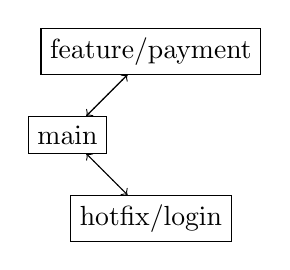
\begin{tikzpicture}[node distance=1.5cm]
\node (main) [draw] {main};
\node (feature) [draw, above right of=main] {feature/payment};
\node (hotfix) [draw, below right of=main] {hotfix/login};

\draw [->] (main) -- (feature);
\draw [->] (main) -- (hotfix);
\draw [->, dotted] (feature) -- (main);
\draw [->, dotted] (hotfix) -- (main);
\end{tikzpicture}
\end{center}

\subsection{高级参数指南}
\begin{center}
\begin{tabular}{@{}ll@{}}
    \toprule
    \textbf{参数} & \textbf{功能} \\
    \midrule
    \texttt{git branch -r} & 仅显示远程分支 \\
    \texttt{git branch -vv} & 显示详细跟踪信息 \\
    \texttt{git branch -f <name> <commit>} & 强制重置分支到指定提交 \\
    \texttt{git branch --track <new> <remote/branch>} & 创建跟踪远程的分支 \\
    \texttt{git branch --set-upstream-to=<remote/branch>} & 修改现有分支跟踪关系 \\
    \bottomrule
\end{tabular}
\end{center}

\subsection{典型工作流应用}
\begin{enumerate}[leftmargin=*, nosep]
    \item \textbf{功能开发流程} \\
    \texttt{\$ git checkout -b feature/search} \quad \textcolor{gray}{// 创建特性分支} \\
    \texttt{\$ git commit -am "实现搜索功能"} \quad \textcolor{gray}{// 在分支开发} \\
    \texttt{\$ git checkout main} \\
    \texttt{\$ git merge feature/search} \quad \textcolor{gray}{// 合并回主分支}
    
    \item \textbf{紧急修复流程} \\
    \texttt{\$ git checkout main} \\
    \texttt{\$ git branch hotfix/security-patch} \\
    \texttt{\$ git checkout hotfix/security-patch} \\
    \texttt{\$ git commit -am "修复安全漏洞"} \\
    \texttt{\$ git push origin hotfix/security-patch}
    
    \item \textbf{分支清理维护} \\
    \texttt{\$ git branch --merged | grep feature/ | xargs git branch -d} \\
    \textcolor{gray}{→ 批量删除已合并的特性分支}
\end{enumerate}

\subsection{分支策略对比}
\begin{center}
\begin{tabular}{@{}lll@{}}
    \toprule
    \textbf{策略} & \textbf{分支类型} & \textbf{适用场景} \\
    \midrule
    Git Flow & 主/开发/特性/发布/热修复 & 正规软件发布流程 \\
    GitHub Flow & 主分支+特性分支 & 持续交付型项目 \\
    GitLab Flow & 生产/预发/特性分支 & 带环境部署流程 \\
    \bottomrule
\end{tabular}
\end{center}

\subsection{最佳实践}
\begin{itemize}[leftmargin=*, nosep]
    \item \textbf{命名规范}:\texttt{feature/}、\texttt{fix/}、\texttt{docs/} 前缀
    \item \textbf{定期清理}:每月删除已合并分支
    \item \textbf{权限控制}:保护主分支禁止直接推送
    \item \textbf{分支生命周期}:特性完成 → 代码评审 → 合并 → 删除
    \item \textbf{可视化工具}:使用 \texttt{gitk} 或 IDE 查看分支拓扑
\end{itemize}

\subsection{问题诊断场景}
\begin{enumerate}[leftmargin=*, nosep]
    \item \textbf{分支游离状态} \\
    \texttt{\$ git status} \quad \textcolor{gray}{// 显示"HEAD detached at..."} \\
    \texttt{\$ git branch temp \&\& git checkout temp} \quad \textcolor{gray}{// 创建临时分支保存}
    
    \item \textbf{远程分支同步} \\
    \texttt{\$ git branch -a} \quad \textcolor{gray}{// 发现远程分支未更新} \\
    \texttt{\$ git fetch origin --prune} \quad \textcolor{gray}{// 同步远程分支状态}
    
    \item \textbf{分支冲突预警} \\
    \texttt{\$ git branch -vv} \\
    \textcolor{gray}{→ [ahead 2, behind 1] 表示需先合并上游修改}
\end{enumerate}


\section{Git 分支功能解析与使用策略}
\textbf{一句话总结:}  
分支是 Git 的核心功能,用于隔离不同开发任务,避免直接修改主代码库,实现高效并行开发与安全实验。

\subsection{分支的核心价值}
\begin{itemize}[leftmargin=*, nosep]
    \item \textbf{任务隔离}:每个功能/修复在独立分支开发,互不干扰
    \item \textbf{风险控制}:实验性代码不会破坏主分支稳定性
    \item \textbf{并行开发}:多人同时处理不同任务
    \item \textbf{版本管理}:通过分支维护不同版本(如生产环境/测试环境)
\end{itemize}

\subsection{分支创建策略}
\begin{center}
\begin{tabular}{@{}lll@{}}
    \toprule
    \textbf{场景类型} & \textbf{分支策略} & \textbf{创建频率} \\
    \midrule
    新功能开发 & 创建 \texttt{feature/} 分支 & 每个功能独立分支 \\
    Bug修复 & 创建 \texttt{hotfix/} 分支 & 每个紧急修复独立分支 \\
    版本发布 & 创建 \texttt{release/} 分支 & 每次大版本发布 \\
    文档更新 & 直接在主分支修改 & 无需单独分支 \\
    小型样式调整 & 直接在主分支修改 & 无需单独分支 \\
    \bottomrule
\end{tabular}
\end{center}

\textbf{核心原则}:
\begin{itemize}[leftmargin=*, nosep]
    \item \textcolor{red}{不推荐}为每次小修改创建分支(增加管理成本)
    \item \textcolor{green}{必需}为以下情况创建分支:
    \begin{itemize}[leftmargin=*, nosep]
        \item 耗时 > 2小时的任务
        \item 影响核心功能的修改
        \item 多人协作的任务
        \item 实验性/高风险变更
    \end{itemize}
\end{itemize}

\subsection{典型场景示例}
\begin{enumerate}[leftmargin=*, nosep]
    \item \textbf{功能开发(需分支)} \\
    \texttt{git checkout -b feature/user-profile} \\
    \textcolor{gray}{→ 开发用户资料功能(耗时3天)} \\
    \texttt{git checkout main} \\
    \texttt{git merge feature/user-profile}
    
    \item \textbf{紧急修复(需分支)} \\
    \texttt{git checkout -b hotfix/login-error} \\
    \textcolor{gray}{→ 修复登录崩溃问题(影响所有用户)} \\
    \texttt{git checkout main} \\
    \texttt{git merge hotfix/login-error}
    
    \item \textbf{文案修改(无需分支)} \\
    \texttt{git checkout main} \\
    \texttt{vim README.md \quad \textcolor{gray}{// 修改文档说明}} \\
    \texttt{git commit -am "更新安装说明"}
\end{enumerate}

\subsection{分支生命周期管理}
\begin{center}
\begin{tikzpicture}
\draw [->] (0,0) -- node[above] {创建分支} (3,0);
\draw [->] (3,0) -- node[above] {开发测试} (6,0);
\draw [->] (6,0) -- node[above] {代码审查} (9,0);
\draw [->] (9,0) -- node[above] {合并主分支} (12,0);
\draw [->] (12,0) -- node[above] {删除分支} (15,0);

\node at (1.5,-0.7) {\texttt{git branch}};
\node at (4.5,-0.7) {\texttt{git commit}};
\node at (7.5,-0.7) {PR/MR};
\node at (10.5,-0.7) {\texttt{git merge}};
\node at (13.5,-0.7) {\texttt{git branch -d}};
\end{tikzpicture}
\end{center}

\subsection{最佳实践指南}
\begin{itemize}[leftmargin=*, nosep]
    \item \textbf{命名规范}:
    \begin{itemize}[leftmargin=*, nosep]
        \item \texttt{feature/search-optimization}
        \item \texttt{hotfix/checkout-error}
        \item \texttt{docs/api-reference}
    \end{itemize}
    
    \item \textbf{分支粒度控制}:
    
\begin{itemize}[leftmargin=*, nosep]
        \item 大型功能 → 拆分子任务分支
        \item 小型修改 → 直接主分支提交
    \end{itemize}
    
    \item \textbf{清理策略}:
    
\begin{itemize}[leftmargin=*, nosep]
  \item 合并后立即删除已完成分支  
  \item 每月清理陈旧分支:\\
    \quad\verb|git branch --merged | grep -v 'main\\|master' | xargs git branch -d|  
\end{itemize}
    \item \textbf{工具支持}:
    
\begin{itemize}[leftmargin=*, nosep]
        \item \texttt{git branch -vv} 查看分支状态
        \item \texttt{git log --graph --oneline} 可视化分支拓扑
    \end{itemize}
\end{itemize}

\subsection{决策流程图}
\begin{verbatim}
                         开始修改
                             ↓
                  [是否影响核心功能?]
                   ↓                   ↓
            是 → 创建新分支        否 → [是否多人协作?]
                   ↓                   ↓           ↓
            [开发/测试]        是 → 创建新分支  否 → [耗时>2小时?]
                   ↓                   ↓                   ↓
            [合并到主分支]      [开发/测试]        是 → 创建新分支
                   ↓                   ↓                   ↓
            [删除分支]          [合并到主分支]      [开发/测试]
                                     ↓                   ↓
                             [删除分支]          [合并到主分支]
                                                      ↓
                                              [删除分支]
\end{verbatim}

\clearpage

\section{Git Merge 功能解析与应用场景}
\textbf{一句话总结:}  
Git Merge 用于将不同分支的修改历史整合到一起,是团队协作和功能集成的核心操作,在代码集成、版本发布和分支同步时发挥关键作用。

\subsection{核心功能解析}
\begin{itemize}[leftmargin=*, nosep]
    \item \textbf{历史整合}:合并两个分支的提交记录
    \item \textbf{变更集成}:将特性分支的修改应用到主分支
    \item \textbf{冲突解决}:提供结构化流程处理代码冲突
    \item \textbf{版本演进}:创建包含多分支变更的新提交
\end{itemize}

\subsection{五大应用场景与触发时机}
\begin{enumerate}[leftmargin=*, nosep]
    \item \textbf{功能开发完成} \\
    \texttt{\$ git checkout main} \\
    \texttt{\$ git merge feature/search} \\
    \textcolor{gray}{→ 将完成测试的搜索功能合并到主分支}
    
    \item \textbf{主分支更新同步} \\
    \texttt{\$ git checkout feature/payment} \\
    \texttt{\$ git merge main} \\
    \textcolor{gray}{→ 避免特性分支偏离主分支太远}
    
    \item \textbf{紧急修复部署} \\
    \texttt{\$ git checkout production} \\
    \texttt{\$ git merge hotfix/security} \\
    \textcolor{gray}{→ 将热修复应用到生产环境}
    
    \item \textbf{版本发布准备} \\
    \texttt{\$ git checkout release/v1.2} \\
    \texttt{\$ git merge develop} \\
    \textcolor{gray}{→ 集成本期所有功能进入发布分支}
    
    \item \textbf{分支策略实施} \\
    \texttt{\$ git checkout main} \\
    \texttt{\$ git merge release/v1.2 --no-ff} \\
    \textcolor{gray}{→ 保留发布分支的合并历史(Git Flow)}
\end{enumerate}

\subsection{合并类型对比}
\begin{center}
\begin{tabular}{@{}lll@{}}
    \toprule
    \textbf{类型} & \textbf{触发条件} & \textbf{结果} \\
    \midrule
    快进合并(Fast-Forward) & 目标分支无新提交 & 不创建新提交 \\
    三方合并(3-Way Merge) & 目标分支有新提交 & 创建合并提交 \\
    递归合并 & 多分支复杂历史 & 自动合并共同祖先 \\
    \bottomrule
\end{tabular}
\end{center}

\subsection{冲突处理流程}
\begin{enumerate}[leftmargin=*, nosep]
    \item 执行 \texttt{git merge} 提示冲突
    \item 使用 \texttt{git status} 定位冲突文件
    \item 编辑文件解决冲突(保留所需代码)
    \item 标记已解决:\texttt{git add <file>}
    \item 完成合并:\texttt{git commit}
\end{enumerate}

\subsection{合并策略选择}
\begin{center}
\begin{tabular}{@{}llp{8cm}@{}}
    \toprule
    \textbf{策略} & \textbf{命令} & \textbf{适用场景} \\
    \midrule
    标准合并 & \texttt{git merge} & 常规分支合并 \\
    压缩合并 & \texttt{git merge --squash} & 清理中间提交 \\
    禁用快进 & \texttt{git merge --no-ff} & 保留特性分支历史 \\
    递归策略 & \texttt{git merge -s recursive} & 复杂分支拓扑 \\
    子树合并 & \texttt{git merge -s subtree} & 合并子项目仓库 \\
    \bottomrule
\end{tabular}
\end{center}

\subsection{最佳实践指南}
\begin{itemize}[leftmargin=*, nosep]
    \item \textbf{预合并检查}:
    \begin{itemize}[leftmargin=*, nosep]
        \item \texttt{git fetch --all} 更新所有分支
        \item \texttt{git diff feature/main} 检查差异
    \end{itemize}
    
    \item \textbf{冲突预防}:
    
\begin{itemize}[leftmargin=*, nosep]
        \item 小批量频繁合并(避免大型合并)
        \item 合并前运行自动化测试
    \end{itemize}
    
    \item \textbf{合并后清理}:
    
\begin{itemize}[leftmargin=*, nosep]
        \item \texttt{git branch -d feature/complete} 移除已合并分支
        \item \texttt{git push --prune} 同步远程分支状态
    \end{itemize}
    
    \item \textbf{可视化工具}:
    
\begin{itemize}[leftmargin=*, nosep]
        \item \texttt{git log --graph --oneline --all}
        \item IDE 内置合并工具(VSCode/IntelliJ)
    \end{itemize}
\end{itemize}

\subsection{典型工作流示例}
\begin{verbatim}
# 开发新支付功能
$ git checkout -b feature/payment
$ git commit -am "支付接口实现"
$ git commit -am "支付页面UI"

# 开发期间同步主分支更新
$ git fetch origin
$ git merge origin/main

# 功能测试通过后合并
$ git checkout main
$ git merge feature/payment

# 处理可能的冲突
$ git mergetool  # 使用可视化工具解决
$ git commit

# 推送到远程
$ git push origin main
\end{verbatim}

\subsection{合并 vs 变基}
\begin{center}
\begin{tabular}{@{}lll@{}}
    \toprule
    \textbf{特性} & \textbf{Merge} & \textbf{Rebase} \\
    \midrule
    历史记录 & 保留原始提交 & 线性重写历史 \\
    适用场景 & 公共分支 & 私有特性分支 \\
    冲突处理 & 单次解决 & 可能多次解决 \\
    使用风险 & 低 & 高(需强制推送) \\
    \bottomrule
\end{tabular}
\end{center}